\section{Client Design}

\subsection{2.2.2 Design of Client Structure}

[intro, with some context goes here (?)]

\subsection{2.2.2.1 Approach}

In designing the client, we had the high level aim of creating a modular system to allow team members to take responsibility for certain aspects of the system. From an early stage in the design process, we were aware that the client had a large set of responsibilities. We determined these responsibilities to be;  to maintain a connection with the server, implement the GIM protocol, provide a user interface to the system and keep a record of up to date information about the user’s friends. Our first task was to design a set of interacting sub-components to handle these responsibilities.

It was agreed that the MVC (Model-Viewer-Controller) architectural pattern, widely used for applications involving a graphical user interface, was a useful model to base our discussions around. This model abstracts the UI (view) from the back end of the system. When a user performs an action, the controller updates a collection of data associated with the system, and updates the interface to reflect any changes the user needs to know about. This seemed appropriate to our needs of keeping and displaying an up to record about the user’s friend list and creating an interface, and would allow us to split responsibilities between the back and front end of the GUI. 

However, we faced challenges in adapting an additional networking component, to implement the GIM protocol, into this framework. We had the choice to conceptually view it as either an additional interface, which ‘viewed’ changes to the model, or indirectly (by way of the network) the controller component. [discussion about possible merits of both goes here] We decided it would be useful to treat the networking code as part of the controller, as it would be modifying the model based on the server’s response to its calls, and modifying the GUI to reflect these changes.
	
This high level approach allowed us to draw high level boundaries between components, and assign the more detailed design of individual components to team members. We decided a logical split would be to assign two members to the networking aspects of the system (client and server), and two members to the GUI components of the system (the GUI and its model.) However, further collaboration was required as it became more evident what was required from each component, from other components, as will be discussed. 

[Diagram goes here, reflecting the above discussion (???) ]

\subsection {2.2.2.2 Model-Viewer-Controller Structural Concerns}

\subsection {Controller}

The controller was one of the more challenging parts of the design process. The controller would be called by both the networking component, and the viewer, implying that its operations must be thread safe. We were constrained by our use of the swing environment, which we had learned from previous experience, will freeze if the networking code is ran on the thread running the GUI. A further complexity was handling the boundary between the requirements of the network code, and the protocol that was being handled by the networking code. Naturally, the GUI architects should not need to concern themselves with the specifics of the protocol, while designing the GUI. 

To deal with the threading complexity, we designed a scheme whereby there would be an intermediate buffer between the controller component, and the networking code. The controller thread would wait until there was a command from the network placed onto the buffer, and act accordingly on the model and GUI. Furthermore, when the controller component needed to call the network, it would place a command onto the buffer, to be interpreted by the  networking code. We believed this scheme to be appropriate as controller could either call the network from internal code, or events from the GUI (possibly simultaneously).

To deal with the design complexity of the boundary, we decided that initially, an interface would be written by the networking architects, including javadoc, to describe the requirements of the GIM protocol of the client, from the controller. In the implementation, the controller would then implement this interface. This allowed the requirements from the client to be understood, without having to understand the inner workings of the protocol. Furthermore, the structure of the protocol could change, without any change to the interface or consultation with the GUI architects. The networking architect would write code to parse incoming commands to calls these methods described by the interface, and write outgoing commands from the GUI.

note: not final version
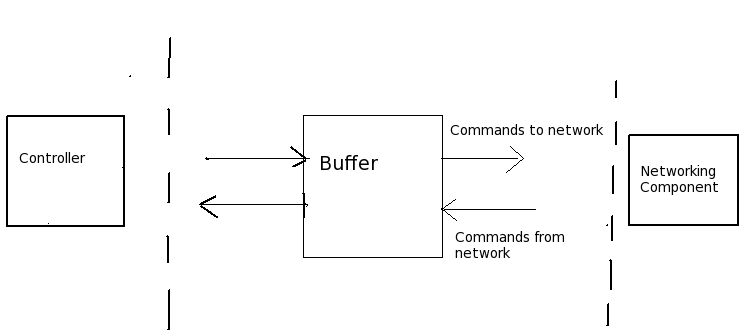
\includegraphics[scale=0.65]{chapter2/diagrams/buffer.png}

\subsection {Model}

The design of the model involved determining what state information had to be held about the client. This was informed by the previous work of requirements analysis and the conception of features. The model was also informed by the design of the viewer.

Two ‘must have’ of the system were the presence of a ‘contact list’, and support for ‘user statuses.’ This implied that there should be data structures for the maintenance of a contact list, and the statuses of users. To deal with this requirement, we designed the model to have a data structure to maintain information about users, including their status, nickname and personal messages. 

The viewer required that the user’s own state information (such as status, and nickname) were displayed. As these were evident in multiple windows in the viewer design (such as in chat windows, and on the buddy list), the model was designed to maintain a record of the user’s current status. 

\subsection {Viewer}

After some interface design work (which will be discussed in coming sections), it was apparent that the system had to support different styles of chat windows for a group chat, and a chat with a single user. However, there was some observable commonality between both windows such as a common need to send messages and display incoming messages, and the swing components handling this functionality. At the same time, there was enough differing behaviour between the two windows, such as the group chat’s need to maintain a list of users in the room, to justify having two different classes to handle them. With this in mind, we designed our class structure code dealing with the interface to have a super class named ChatWindow, outlining this common functionality, which two sub classes called GroupChatWindow and SingleChatWindow which would extend this super class. 

We anticipated this would be advantageous as it would reduce the repetition of code, and keep functionality consistent between the two windows. We felt in particular the panel displaying incoming images would change in formatting messages, as the project would evolve to include some of our possible features, such as the implementation of emoticons and font colours (See section x.y).  

[CLASS DIAGRAM REPRESENTATION]








\subsubsection{}





